\chapter{Challenges for design of applications}

The biggest design challenge for developers of gesture controls is market adoption, standardization and application design.

\section{Market Adoption}

\subsection{Myo Armband}

\begin{wrapfigure}{r}{0.5\textwidth}
  \begin{center}
    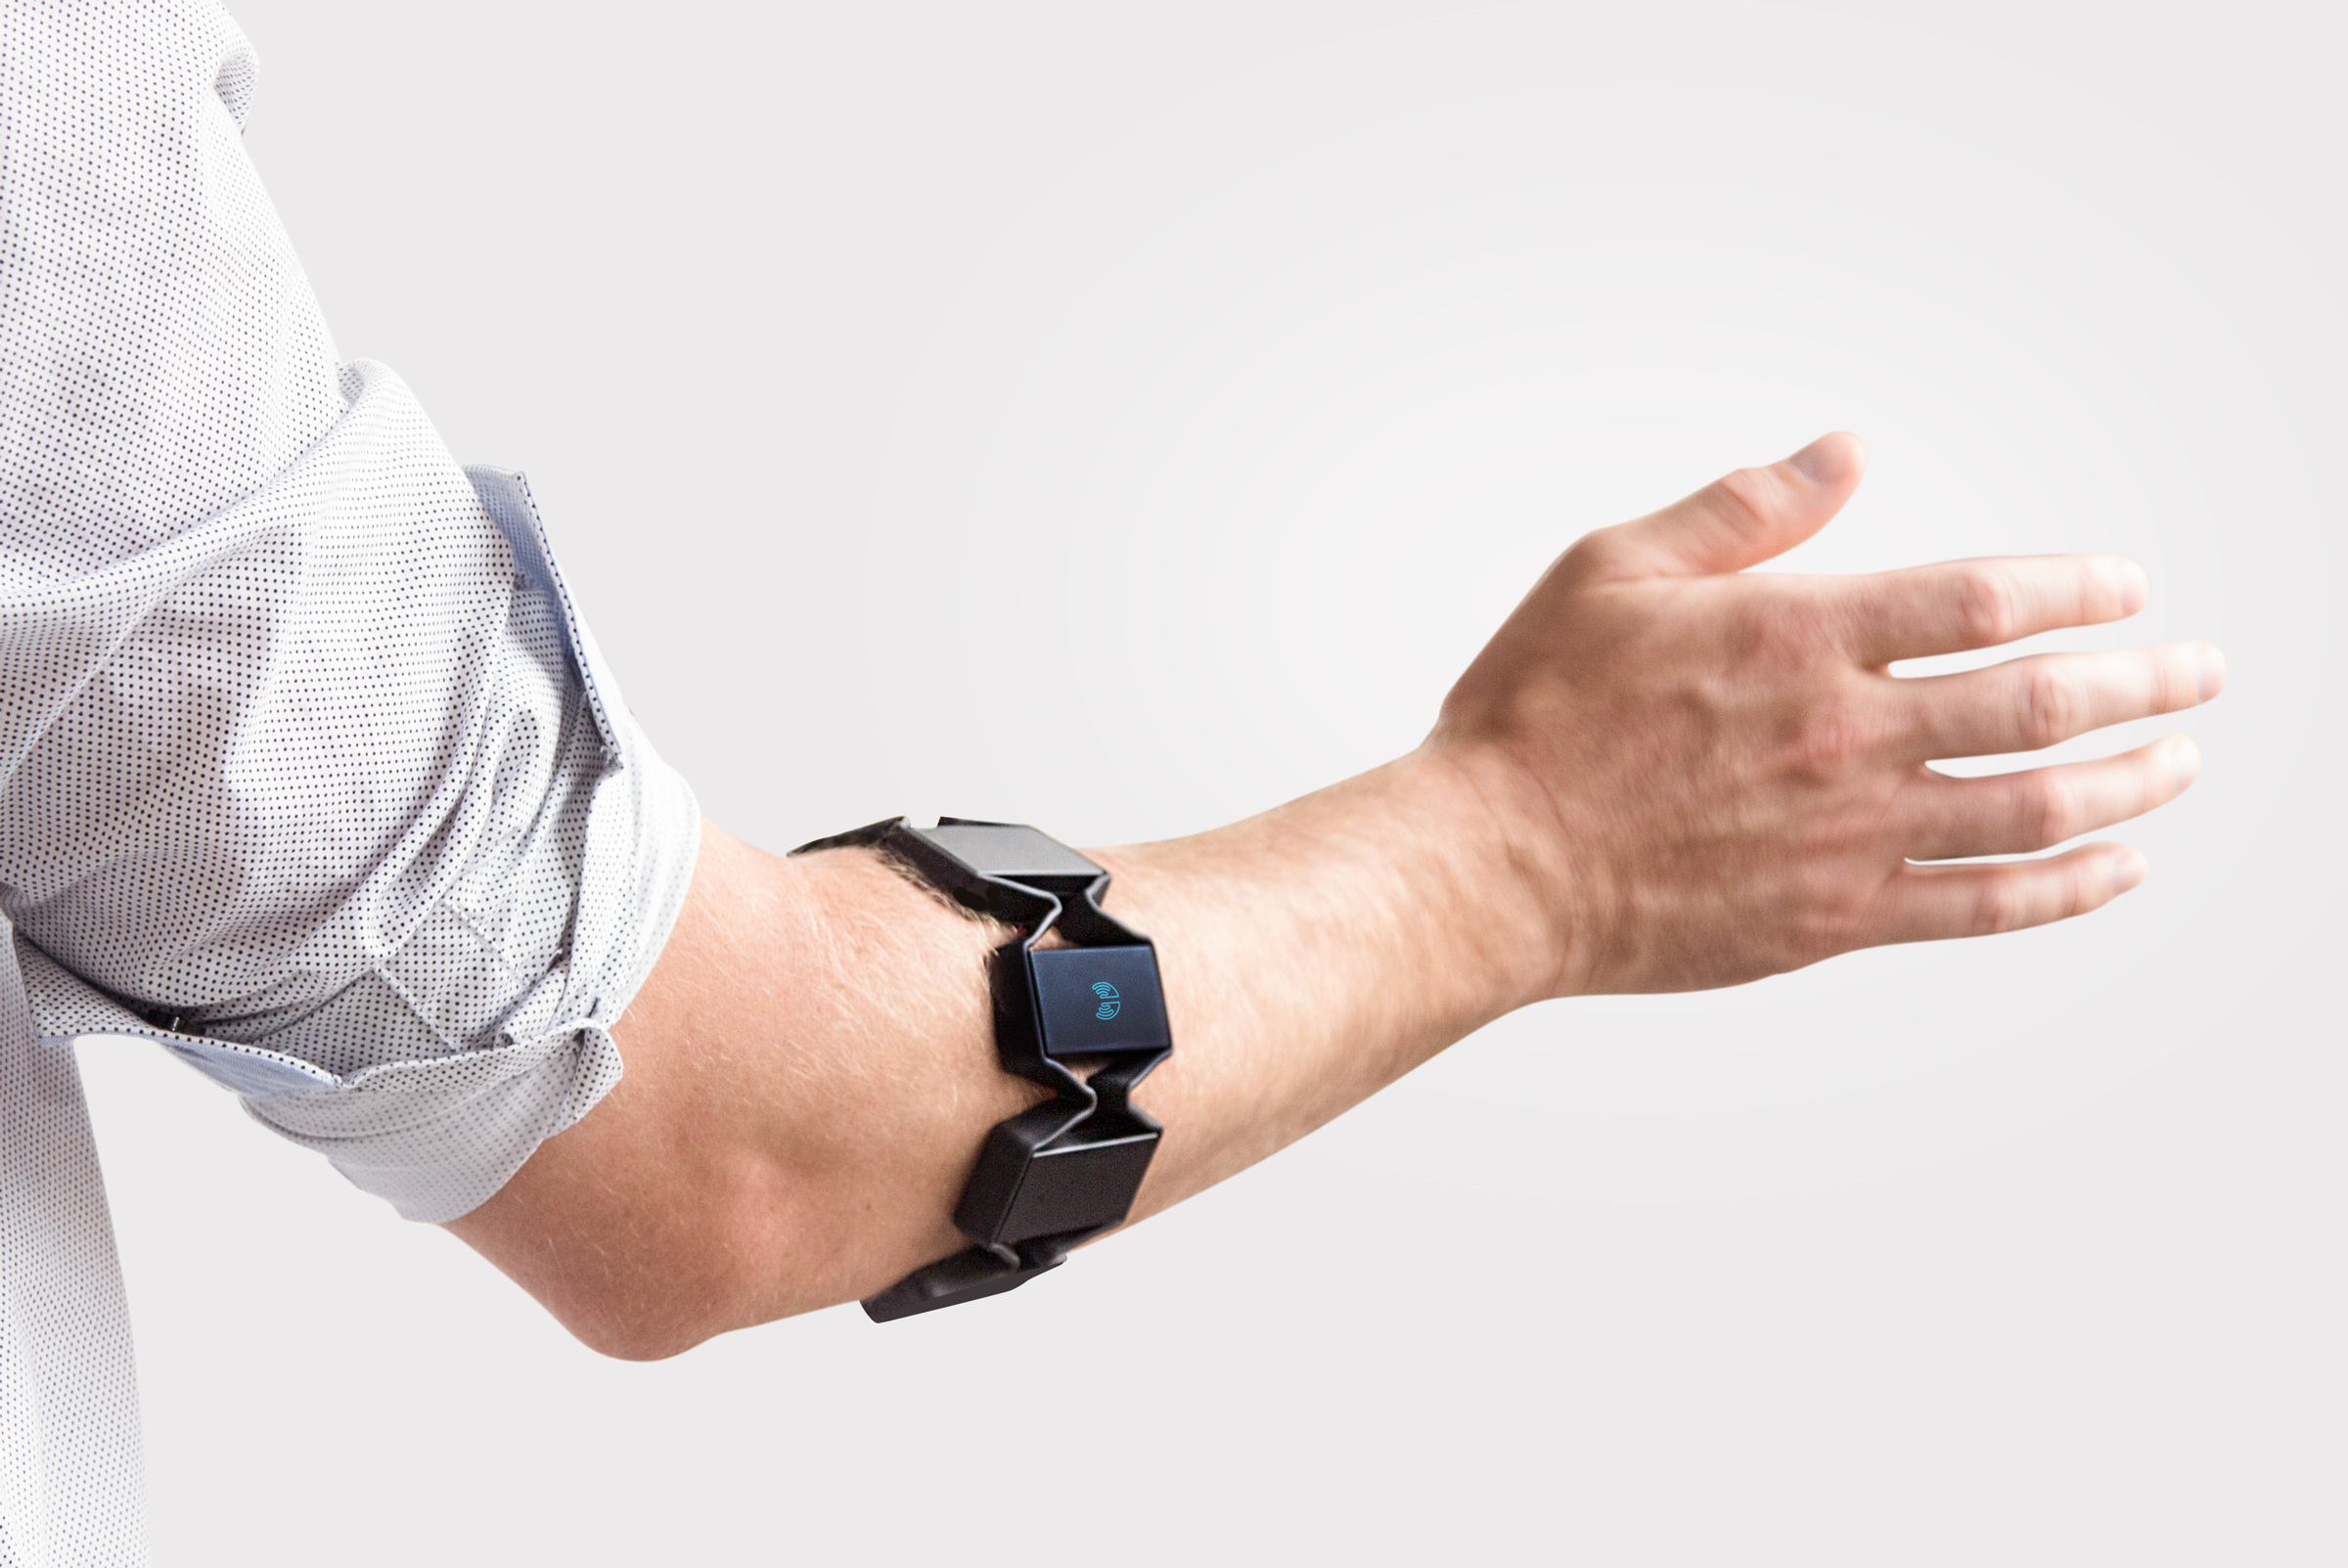
\includegraphics[width=0.48\textwidth]{img/myo.jpg}
  \end{center}
  \caption{Myo Armband}
\end{wrapfigure}

One of the biggest challenges of gesture based technology is market adoption. If the technology isn't adopted by a large segment of the population developers mostly ignore it in favor of bigger market, such as mobile phones and the traditional desktop.

Devices like the Myo armband started out with great success raising 14.5 Million dollars in 2013 with 30,000 pre-orders for their product. The problem started with lackluster support from developers who weren't as supportive of the technology as the customers were. \cite{myosales}

Devices like Myo Armband suffered due to developer support which caused customers to lose interest with the technology.

\subsection{Kinect}

Even industry giant Microsoft tried to break into the gesture controls space with the introduction of the Kinect back in 2010. \cite{kinect} The Kinect was Microsoft's attempt of adding gesture controls to their gaming console the Xbox 360. With support from Microsoft many developers made Kinect only games (Kinect Sports, Kinect Adventures!, Kinectimals) and other added Kinect support (Elder Scrolls: Skyrim, Forza Motorsports 4). With support from Microsoft the Kinect looked to be on the rise as sales reached 10 Million. \cite{kinectsales}

\begin{figure}[H]
  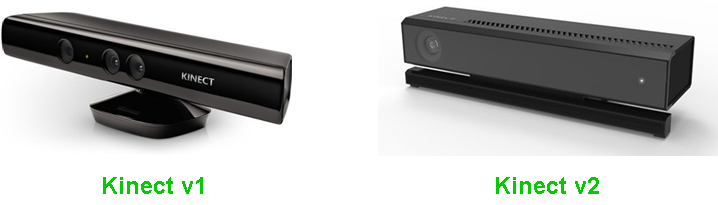
\includegraphics[width=\linewidth]{img/Kinect.png}
  \caption{Kinect V1/2}
  \label{fig:KINECT}
\end{figure}

From 2010 (Release of Kinect V1) to 2013 (Release of Kinect V2) customers opinion had changed on the kinect. Many felt the kinect games felt gimmicky' and games that added kinect support didn't make using it over a traditional controller better. This dislike of gesture controls came to ahead with the release of the Xbox One, which originally was debuted with a new Kinect, which had to be plugged in at all times. With a price tag 100 dollar more than their competition many blamed the Kinect for this price difference. 

With the Xbox One release having a Kinect market adaption should have been even better than the previous iteration of the kinect. Unfortunately the announcement of the Xbox One was  a disaster causing lots of controversy that was then directed towards the Kinect. The Kinect got lackluster support and many had concern of privacy with an always on camera and speaker. The Kinect was dropped in later models of Xbox Ones with users having to buy an adapter to get one to work with the newer models. This adapter was then dropped leaving users who enjoyed the connect behind.

\section{Standardization}



%% Talk about gestures having different meaning around the world